\documentclass{article}
\usepackage[utf8]{inputenc}
\title{video 3:geometric analysis of covariance }
\author{wbg231 }
\date{December 2022}
\newcommand{\R}{$\mathbb{R}$}
\newcommand{\B}{$\beta$}
\newcommand{\A}{$\alpha$}
\newcommand{\D}{\Delta}

\newcommand{\avector}[2]{(#1_2,\ldots,#1_{#2})}
\newcommand{\makedef}[2]{$\textbf{#1}$:#2 }
\usepackage{tikz,graphicx,hyperref,amsmath,amsfonts,amscd,amssymb,bm,cite,epsfig,epsf,url}

\begin{document}

\maketitle

\section{introduction}
\begin{itemize}
\item\href{https://www.youtube.com/watch?v=-sIvLCXcliE&t=298s}{video link}
\item here we are thinking of random variables as vectors in a vector space
\item keep in mind that vectors are more abstract than just the cs notion of vectors as lists of numbers
\item properties of a vector
\begin{itemize}
    \item vector addition must be communicative and associative
    \item vectors must be saleable by any real number
\end{itemize}
\item properties of a vector space $V$
\begin{itemize}
    \item closed under scalar multiplication ie $\forall \beta \in \mathbb{R}. b\in V \beta v\in V$
    \item closed under vector addition 
    \item there needs to be a zero vector such that $\forall x\in V x+0=x$
    \item there must always be an inverse ie $\forall x \in V \exists -x : x+(-x)=0$
    \item if some set of objects meet these conditions they are a vector space
\end{itemize}
\item the random variables are a vector space
\section{vector space for random variables}
\item when are two random variables a and b equal
\item it is not when they have the same distribution instead it is when $P(a=b)=1$
\item call the vector space of random variables $R$
\item random variables are clearly closed under scalar multiplication and vector addition 
\item the random variable 0 such that $P(0=0)=1$ is the zero in this space
\item further we can see that for any random variable a there exists an inverse $-a\in R$ such that $-a=-1(a)$ meaning $a+(-a)=0$
\section{inner product}
\item the inner product $<*,*>$ allows us to think about angles
\item an inner product is valid if 
\begin{itemize}
    \item it is symmetric that is $\forall v_1,v_2\in R$ we have $<v_1,v_2>=<v_2,v_1>$
    \item and linear that is $\forall \beta \in \mathbb{R}, v_1,v_2,v_3\in R$ we have $<\beta v_1,v_2>=\beta <v_1,v_2>$ and $<v_1+v_3,v_2>=<v_1,v_2>+<v_3,v_2>$ 
    \item we also want the inner product to be positive semi definite ie $\forall v <v,v>\geq0$ and $<v,v>=0 \iff v=0$
\end{itemize}
\section{covariance as an inner product}
\item covariance is a valid inner product if we have zero mean random variables 
\item remember that $cov(a,b)=E[ab]-E[a]E[b]$ if all rvs have zero mean than $cov(a,b)=E[a]E[b]$ so this makes sense as the covariance in this context is effectively a product of the means of each random variable 
\item showing covariance is an inner product
\begin{itemize}
    \item first we want to show covariance is symmetric $cov(a,b)=E[ab]=E[ba]=cov(b,a)$
    \item linear part 1 $cov(\beta a, b)=E[\beta a*b]=\beta E[ab]=\beta cov(a,b)$
    \item linear part 2 $cov(a+c,b)=E[(a+c)b]=E[ab+cb]=e[ab]+e[cb]=cov(a,b)+cov(c,b)$
    \item now we want to show positive semi definiteness first assume that $cov(a,a)=0$ this implies that $E[a^2]=0$ which implies $P(a=0)=1$ thus $a=0$ this is why we need zero mean random variables, now assume $a=0$ we know that $P(a=0)=1$ implying $E[a]=0$ and we can see $E[a^2]=\Sigma_{a\in A}aP(a=a)=0(1)=0$ and that $cov(a,a)=E[a^2]=0$ 
    \item so covariance of mean zero ie centred random variables is indeed a valid inner product. 
\end{itemize}
\section{norm of a vector}
\item the norm is the length of a vector. 
\item the norm induced by an inner product is $||V||=\sqrt{<v,v>}$
\item so for a mean zero random variable $a$ we Can say $||a||=\sqrt{cov(a,a)}=\sqrt{E[a^2]-e[a]^2}=\sqrt{var(a)}=\sigma_{a}$ 
\item so in this vector space the length of a random variable is it's standard variance
\section{angle between vectors}
\item recall in general the cosine of the angle between two vectors $a,b$ is given by $cos(\theta)=\frac{<a,b>}{||a||||b||}$ in other words it is there inner product normalized by there length
\item so in our random variable vector space we can see $cos(\theta)=\frac{<a,b>}{||a||||b||}=\frac{cov(a,b)}{\sqrt{var(a)var(b)}}=\rho_{a,b}$ in other words the correlation coefficient is the cosine of the Angel between two random variables 
\section{picture}
\item 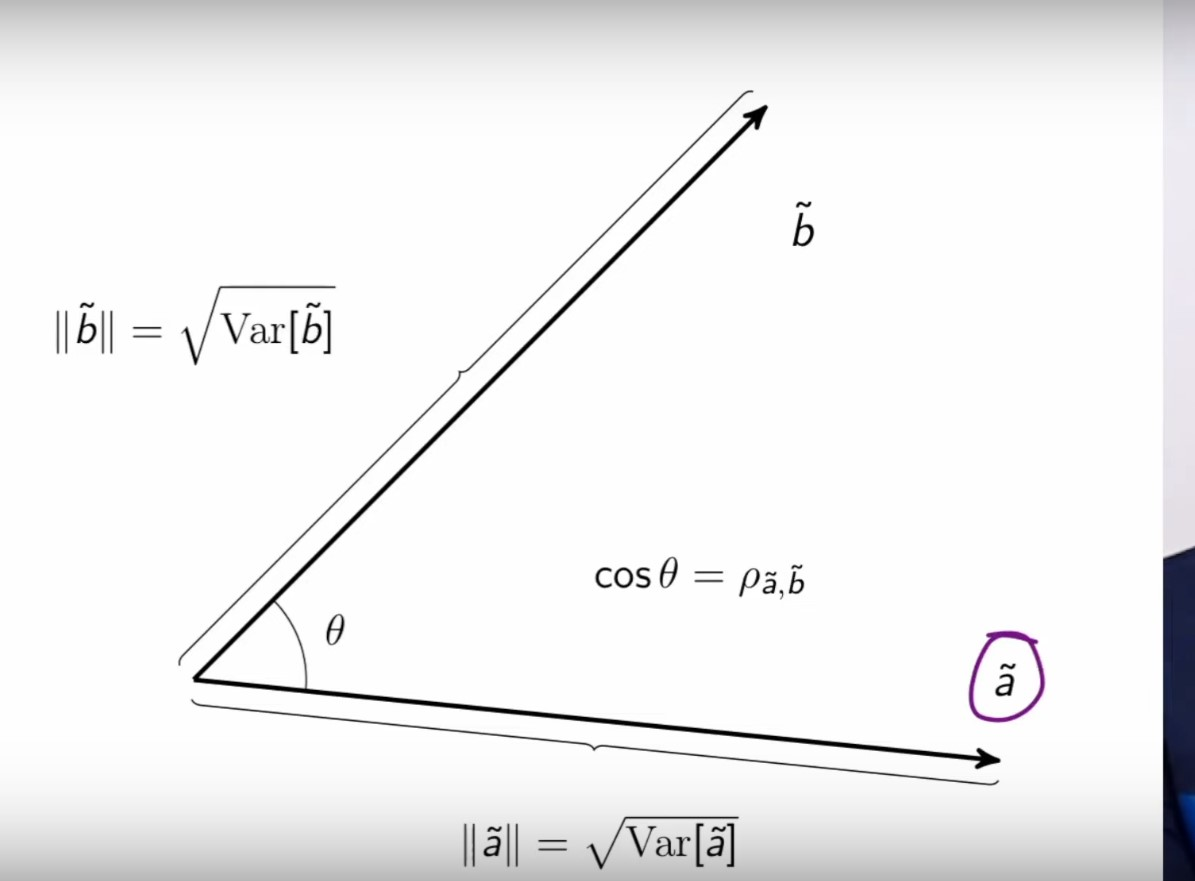
\includegraphics[width=10cm]{notes/week_2/geometric_1.jpg}
\item so the above picture has all the stuff we talked about
\item the length of vectors are there standard deviation 
\item the cosine of the angle between vectors are there coefficient of correlation 

\section{insights from this analysis}
\item first as we know $cos(\theta)\in [-1,1]$ we know $\rho_{a,b}\in [-1,1]$
\item if $\rho_{a,b}>0$ it means the vectors are positively correlated and thus $cos(\theta)>0$ meaning a and b are pointing in the same direction 
\item if $cos(\theta)=0$ then $\rho_{a,b}=0$ meaning they are independent or orthogonal 
\item if $cos(\theta)=\pm 1$ geometrically a and b are co linear and $\rho_{a,b}=\pm 1$ meaning they have perfect liner correlation ie they are linear dependant
\item so this analysis captures a lot of the properties of $\rho_{a,b}$ quite simply
\section{simple linear regression}
\item within the vector space of random variables as we have defined it what if we want to use a to linearly estimate b. 
\item 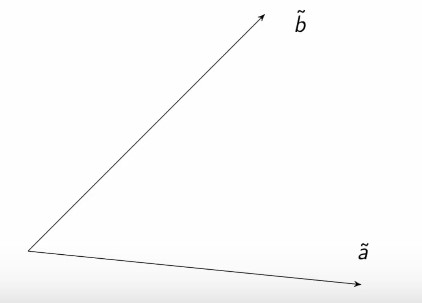
\includegraphics[width=10cm]{notes/week_2/geometric_2.jpg}
\item so we want to think how much do we have to scale a to obtain the best possible estimate for b 
\item so this problem is equivalent to finding the best scalar $\beta \in \mathbb{R}$ which minimizes the distance between $\beta a, b$
\item recall in our vector space the length of a vector v is given by it's standard deviation that is length is $||v||=\sqrt{var(v)}=E[v^2]-E[v]^2=E[v^2]$ because we are in mean zero space
\item so finding the best linear estimate within this space is equivalent to minimizing the distance between a and $\beta a$ which is equivalent to minimizing the length of there difference that is $||b-\beta a||=\sqrt{var(b-\beta a)}=\sqrt{E[(b-\beta a)^2)]-E[b-\beta a]^}2=\sqrt{E[(b-\beta a)^2)]}$ 
\item so we can further write $E[(b-\beta a)^2]=var[b-\beta a]=||b-\beta a||^2$that is mean squared error is length squared in this vector space
\item in order to minimize that distance we need the closest point to b that lies on a. 
\item the point that is closest to b on a is the orthogonal projection of b onto a. 
\item so in other words we want $b-\beta a \perp a $ meaning that $<a,b-\beta a>=cov(b-\beta a,a)=0$
\item this works out to$\beta=\frac{<a,b>}{||a||^2}=\frac{cov(a,b)}{var(a)}=\frac{cov(a,b)}{\sqrt{var(a)var(b)}}\frac{\sqrt(var(a)}{\sqrt{var(b)}}=\rho_{a,b}\sqrt{\frac{var(a)}{var(b)}}=\rho_{a,b}\sigma_{b}\frac{1}{\sigma_{a}}$
\item so if we write $\beta a=\sigma_{b}\rho_{a,b}\frac{a}{\sigma_{a}}=l(a)$ ie the min mean squared error estimator for mean zero random variables
\section{residuals}
\item 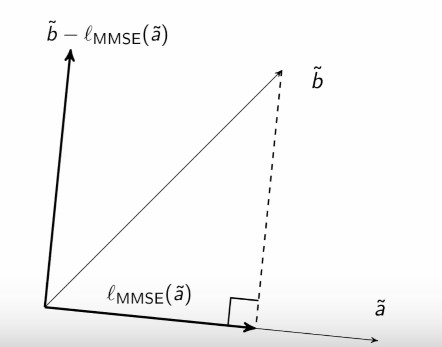
\includegraphics[width=10cm]{notes/week_2/geometric_3.jpg}
\item note from this we can see that the residual $b-l(a)$ is orthogonal to l(a), a
\item this is the same as what we saw earlier 
\section{Pythagoras theorem }
\item so note that $b=(l(a))+(b-l(a))$ and that$(b-l(a))\perp(l(a))$ meaning we can apply Pythagoras theorem to say  $||b||^2=var(b)= var(l(a))+var(b-l(a))$
\item so this gives us the decomposition of variance that we saw earlier 
\item ie that the variance of b is equal to the sum of the variance of the linear estimator and it's residual 
\section{length of the projection}
\item recall that $||l(a)||^2=||\beta a||^2=var(\beta a)=\beta^2var(a)=\frac{rho_{a,b}^2var[b]}{var[a]}=\rho_{a,b}^2var(b)$
\item this allows us to rederrive $R^2=\rho_{a,b}^2$ as $\frac{||l(a)||^2}{||b||^2}=\frac{var(l(a)}{var(b)}=\frac{\rho^2var(b)}{var(b)}=\rho_{a,b}^2=R^2$ so this can still be interpreted as the percentage of variances in b explained by the linear estimator 
\end{itemize}

\end{document}
